\section{Theorie}
	
Im Folgenden sollen zunächst die theoretischen Grundlagen für die nachfolgenden experimentellen Untersuchungen erörtert werden.
Die vorgestellte Theorie basiert auf der ausgehändigten Versuchsanleitung \cite{wwu}.

\subsection{Schalenmodell des Kerns}

Das Schalenmodell des Atomkerns ist sehr ähnlich zum Fermigasmodell. Wesentlicher Unterschied zum Fermigasmodell ist das abgeänderte Kernpotential. Anstelle eines Rechteckpotentials wird ein Woods-Saxon-Potential genutzt:
\begin{align*}
	V(r)=\frac{-V_0}{1+\exp\left( \frac{r-R}{a}\right) }
\end{align*}
Dabei bezeichnet $V_0$ die Potentialtiefe, $a$ die Ausschmierung des Kernrandes, $R$ den Kernradius und $r$ den Abstand des Nukleons vom Kernmittelpunkt. Außerdem wird die Spin-Bahn-Kopplung der Nukleonen berücksichtigt, denn wie Elektronen im Atom besitzen auch Nukleonen im Kern einen Bahndrehimpuls und einen Spin. Insgesamt ergeben sich die in Abbildung \ref{schalen} dargestellten Energieniveaus. 

Dieses Schema der möglichen Zustände erinnert an die Energieniveaus eines Atoms, was den Namen \glqq Schalenmodell\grqq\ erklärt. Außerdem sind in Kästchen die \emph{magischen Zahlen} eingezeichnet. Wenn alle Zustände bis zu einer größeren Energielücke besetzt sind, erhält man eine Art \glqq Schalenabschluss\grqq, was die ungewöhnlich hohe Bindungsenergie der Kern bei den magischen Zahlen erklärt. Dieses Phänomen konnte mit früheren Modellen nicht ausreichend erklärt werden.

\begin{figure}[h]
	\centering
	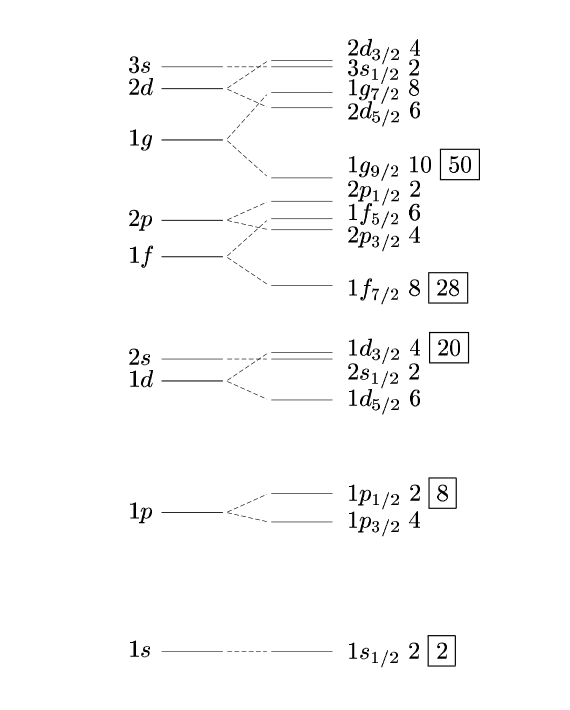
\includegraphics[width=0.6\textwidth]{img/schalen}
	\caption{Energieniveaus des Schalenmodells. Die Spin-Bahn-Kopplung ist hier explizit berücksichtigt. \cite{schalen}}
	\label{schalen}
\end{figure}

\subsection{Emission von $\gamma$-Strahlung}

Nach $\alpha$- und $\beta$-Zerfällen liegen die die Kerne oft in einem angeregten Zustand vor. Die \glqq Abregung\grqq\ geschieht meist über die Aussendung von $\gamma$-Quanten, also hoch-energetischen Photonen. Im Gegensatz zu den elektromagnetischen Übergängen in der Atomhülle, wo fast nur Dipolstrahlung auftritt, sind bei den Übergängen im Kern höhere Multipole (Quadrupol, Oktupol, ...) nicht zu vernachlässigen. 

Statt der Emission von Photonen kann die Energie auch an ein Elektron in der Hülle des Atoms abgegeben werden, welches dadurch aus dem Atom herausgeschlagen wird (Konversionselektronen). Im Gegensatz zur $\beta$-Strahlung entstammen diese jedoch nicht dem Kern selbst und besitzen außerdem ein diskretes Energiespektrum. Bei sehr hohen Energien ist zudem die Bildung und Emission eines Elektron-Positron-Paares im Kern möglich (Paarkonversion).

\subsubsection{Auswahlregeln und Multipolstrahlung}

Bei elektromagnetischen Übergängen muss der Gesamtdrehimpuls erhalten bleiben. Besitzt das emittierte Photon den Drehimpuls $l$ und die beteiligten Kernniveaus die Drehimpulse $I_i$ und $I_f$, dann muss gelten:
\begin{align}
	\left| I_i - I_f\right| \leq l \leq I_i + I_f
\end{align}
Man unterscheidet nun zwischen elektrischer (E$l$) und magnetischer (M$l$) $2^l$-Strahlung (Bsp. $l=1\Longrightarrow$ Dipolstrahlung, $l=2\Longrightarrow$ Quadrupolstrahlung, ...). Mit steigendem $l$ nimmt die Wahrscheinlichkeit für einen solchen Übergang exponentiell ab.

Es lässt sich nun zusätzlich die Paritätsquantenzahl $P=\pm 1$ definieren, welche das Symmetrieverhalten einer Wellenfunktion unter einer Koordinatentransformation $\vec{x}\longrightarrow -\vec{x}$ beschreibt. Es gilt für die Parität von Anfangs- und Endzustand ($P_i$ und $P_f$):
\begin{align}
	\Delta P= P_i\cdot P_f = \begin{cases}
	\left( -1\right)^l\,\,\,\,\,&\text{für E$l$-Strahlung} \\
	\left( -1\right)^{l+1}\,\,\,\,\,&\text{für M$l$-Strahlung}
	\end{cases}
\end{align}

\subsubsection{Winkelverteilung bei $\gamma$-$\gamma$-Kaskaden}

Ausgangspunkt zur Berechnung der theoretisch erwarteten Winkelverteilung ist die Überlegung, dass der Detektor im Vergleich zur Ausdehnung der Quelle sehr weit von dieser entfernt ist (Details im Versuchsaufbau). Das hier nur klassisch betrachtete elektromagnetische Feld kann daher näherungsweise als quellfrei angenommen werden. Die Maxwell-Gleichungen vereinfachen sich daher zu:
\begin{align}
	\begin{split}
		\vec{\nabla}\times\vec{E}=-\frac{\partial B}{\partial t}\qquad\qquad \vec{\nabla}\times\vec{B}=\frac{1}{c^2}\frac{\partial E}{\partial t}\\\vspace{0,2cm}
		\vec{\nabla}\cdot\vec{E}=0 \,\,\qquad\qquad\qquad\vec{\nabla}\cdot\vec{B}=0\qquad\;
	\end{split}
\end{align}
Die Lösungen sind gegeben durch:
\begin{align}
	\begin{split}
		\vec{B}^m_l= f_l(kr)\cdot\vec{L}\cdot Y^m_l(\Theta,\Phi)\qquad ; \qquad \vec{E}^m_l = i \frac{c}{k} \cdot\vec{\nabla}\times \vec{B}^m_l\qquad\text{für $E$-Felder}\\
		\vec{E}^m_l= f_l(kr)\cdot\vec{L}\cdot Y^m_l(\Theta,\Phi)\qquad ; \qquad \vec{B}^m_l = -i \frac{c}{k} \cdot\vec{\nabla}\times \vec{E}^m_l\qquad\text{für $M$-Felder}
	\end{split}
\end{align}
Die Ausstrahlungscharakteristik ist durch den Poynting-Vektor $\vec{S}=\frac{1}{\mu_0}\left( \vec{E}\times\vec{B}\right) $ gegeben. Im Fernfeld gilt:
\begin{align}
	\epsilon_0\left| \vec{E}\right| ^2=\frac{1}{\mu_0}\left| \vec{B}\right| ^2
\end{align}
Damit folgt für die Winkelverteilung insgesamt:
\begin{align}
\begin{split}
\left|\vec{S} \right| \sim \left| \vec{E}\right|^2 \sim \left| \vec{L}\cdot Y^m_l\right|^2\qquad\text{für $E$-Felder}\\
\left|\vec{S} \right| \sim \left| \vec{B}\right|^2 \sim \left| \vec{L}\cdot Y^m_l\right|^2\qquad\text{für $M$-Felder}
\end{split}
\end{align}
Das heißt, über die Kugelflächenfunktionen $Y^m_l(\Theta,\Phi)$ lässt sich die Winkelverteilung berechnen. Für die hier untersuchten $\gamma$-Kaskade beim Zerfall von $^{60}_{27}$Co in $^{60}_{28}$Ni erwartet man:
\begin{align}
	W(\Theta)\sim 1+\frac{1}{8}\cos^2(\Theta)+\frac{1}{24}\cos^4(\Theta)
\end{align}
Damit lässt sich auch die theoretisch erwartete Asymmetrie berechnen:
\begin{align}
	A_\text{theo.}=\frac{W(180\text{°})-W(90\text{°})}{W(90\text{°})}
\end{align}
Aus der gemessenen Koinzidenzrate bei den jeweiligen Winkeln lässt sich analog die experimentelle Asymmetrie berechnen und mit der theoretischen vergleichen:
\begin{align}
A_\text{exp.}=\frac{C(180\text{°})-C(90\text{°})}{C(90\text{°})}
\end{align}
\subsubsection{Wechselwirkung von Photonen mit Materie}

Ein weiterer wichtiger Punkt ist die Absorption von Photonen in Materie. Es gibt drei verschiedene Prozesse zur Absorption von Photonen, die für unterschiedliche Energiebereiche dominant sind:

\begin{description}
	\item[Photoeffekt:]\hfill
	dominant im eV- bis keV-Bereich
	
	Die gesamte Energie des Photons wird auf ein Elektron in der Hülle der Atome des Absorbermaterials übertragen. Dieses Elektron verlässt das Atom und trägt die bei der Ionisation überbleibende Energie als kinetische Energie davon und kann dadurch weitere Atome ionisieren. Der Wirkungsquerschnitt ist proportional zu $Z^5/E_\gamma^3$ ($Z$: Kernladungszahl des Absorbermaterials, $E_\gamma$: Energie der Photonen).
	
	\item[Comptonstreuung:]\hfill 
	dominant im MeV-Bereich
	
	Das Photon wird an einem quasi freiem Elektron gestreut. Der Energieübertrag ist dabei vom Streuwinkel abhängig. Bei einem Winkel von 0° ist der Energieübertrag null, bei einem Winkel von 180° (Rückstreuung) ist er maximal.
	
	\item[Paarproduktion:]\hfill 
	dominant bei Energien über 10\,MeV
	
	Im elektrischen Feld eines Atomkerns  kann die Energie des Photons dazu genutzt werden, um ein Elektron-Positron-Paar zu erzeugen. Dies kann aber offensichtlich nur dann passieren, wenn die Photonenergie die Summe der Ruhemassen von Elektron und Positron (1022\,keV) übersteigt.
\end{description}

\subsection{Positronium}

Trifft ein bei einem $\beta^+$-Zerfall emittiertes Positron auf Materie, so gibt es zunächst durch Stöße mit den enthaltenen Elektronen Energie ab. Ist die Energie des Positrons so weit verringert, dass es thermalisiert ist, kann es entweder mit einem der Elektronen des Materials sofort annihilieren, oder Elektron und Positron gehen in einen gebundenen Zustand, dem Positronium über. Man unterscheidet dabei zwei Arten des Positroniums:

\begin{description}
	\item[Parapositronium:]\hfill
	
	Die Spins von Elektron und Positron sind antiparallel ausgerichtet, es handelt sich also um einen Singulett-Zustand. Es zerfällt mit einer Lebensdauer von 125\,ps meist in zwei 511\,keV Photonen, die sich im 180°-Winkel zueinander ausbreiten. Dies ist der für den Versuch relevante Zustand.
	
	\item[Orthopositronium:]\hfill 
	
	Dies ist der Tripltett-Zustand des Positroniums, die Spins von Elektron und Positron sind parallel ausgerichtet. Es zerfällt mit einer Lebensdauer von 140\,ns in mindestens drei Photonen.
	
\end{description}

\subsection{Szintillatoren}

Bei der Detektion von Gamma-Strahlung ist es zumeist notwendig, die Energie der Photonen soweit zu verringern, dass die Wellenlänge nachher im sichtbaren Bereich liegt. Diese Aufgabe erfüllen Szintillatoren. Treffen hoch-energetische Gamma-Quanten auf das Absorbermaterial des Szintillators, so geben sie über den Comptoneffekt Energie an das Material ab. 

Man unterscheidet zwischen anorganischen Szintillatormaterialien, welche eine hohe Wechselwirkungsrate haben, aber auch eine große Ansprechzeit, und organischen (Plastik-)Szintillatoren, welche weniger mit einfallender Strahlung wechselwirken und dafür schneller ansprechen. Entsprechend eignen sich anorganische eher zur Detektion von Gamma-Strahlung und organische eher für massive Teilchen (Alpha-Teilchen, Spaltbruchstücke, ...). 

In dieser Versuchsreihe werden anorganische Szintillatoren verwendet. Diese besitzen eine Kristallstruktur und können demnach durch das Bändermodell verstanden werden. Gibt ein eintreffendes Photon Energie an eines der Elektronen des Szintillatormaterials ab, so wird dieses in das Leitungsband angehoben, beim Driftprozess kann dieses Elektron dabei weitere Atome ionisieren. 

Entscheidend ist nun, dass bei der Abregung eine geringere Bandlücke überwunden wird als bei der Anregung, sodass die ausgesandten Photonen keine erneute Anregung der Valenzelektronen bewirken können und der Szintillator somit für die Photonen transparent erscheint. Diese Übergänge mit niedriger Energiedifferenz können durch eine geeignete Dotierung erzeugt werden. Die überschüssige Energie wird dabei z.B. durch Gitterschwingungen (Phononen) abgegeben. Die Anzahl der erzeugten Photonen, welche im sichtbaren Wellenlängenbereich liegen, ist proportional zur Energie des einfallenden Gamma-Quants, wodurch diese mithilfe von nachgeschalteten Photomultipliern leicht bestimmt werden kann.


\subsection{Photomultiplier}

Photomultiplier eignen sich zur Detektion einzelner Photonen im sichtbaren Wellenlängenbereich. Damit sie auch ionisierende Strahlung detektieren können, ist ihnen ein Szintillator vorgeschaltet. Die Detektion von Photonen geschieht dabei über den Photoeffekt, bei dem ein eintreffendes Photon ein Elektron aus einer Dynode herauslöst. Da ein einzelnes Elektron nicht als ein ausreichend starker Strom gemessen werden kann, wird mittels einer Beschleunigungsspannung das Elektron auf eine weitere Dynode gelenkt, wo es neue Elektronen herauslösen kann. Dieser Vorgang wird solange wiederholt, bis die Verstärkung groß genug ist, dass ein ausreichender Spannungspuls detektiert werden kann.